%\documentclass[12pt,letterpaper,twoside]{article}
\documentclass[12pt,letterpaper]{article}
\usepackage{amsmath}
\usepackage{amsfonts}
%\usepackage{appendix}
\usepackage[figurewithin=section,tablewithin=section]{caption}
\usepackage[usenames,dvipsnames]{color}
\usepackage{graphicx}
\usepackage{longtable}
\usepackage{rotating}
%\usepackage{verbatim}
\usepackage[pdftex,bookmarksopen=false]{hyperref}
%\usepackage[pdftex]{hyperref}
\hypersetup{pdfauthor={John Sibert}}
\hypersetup{pdfsubject={Yellowfin stock assessment}}
\hypersetup{pdftitle={Assessment of the yellowfin tuna Thunnus albacares 
stock in the Main Hawaiian Islands Yellowfin Tuna Fishery}}
\hypersetup{pdfkeywords={yellowfin tuna,state space model,stock assessment,Hawaii}}

\newcommand\doublespacing{\baselineskip=1.6\normalbaselineskip}
\newcommand\singlespacing{\baselineskip=1.0\normalbaselineskip}
\renewcommand\deg[1]{$^\circ$#1}
\newcommand\SD{SEAPODYM}
\newcommand\MFCL{MULTIFAN-CL}
\newcommand\ADMB{ADModel Builder}
\newcommand\SPC{Secretariat of the Pacific Community}
\newcommand\WCPO{Western Central Pacific Ocean}
\newcommand\WCPFC{Western Central Pacific Fisheries Commission}
\newcommand\SSAP{Skipjack Survey and Assessment Programme}
\newcommand\RTTP{Regional Tuna Tagging Programme}
\newcommand\PTTP{Pacific Tuna Tagging Programme}
\newcommand\FAD{fish aggregating device}
\newcommand\ADRM{advection-diffusion-reaction model}
\newcommand\help[1]{\color{Magenta}{\it #1}\normalcolor}
\newcommand\widebar[1]{\overline{#1}}
\newcommand\EEZ{Exclusive Economic Zone}

\newcommand\None{{N_{1,1}}}
\newcommand\Ntwo{{N_{2,1}}}
\newcommand\Nsum{{N_{1,1}+N_{2,1}}}
\newcommand\peryr{yr$^{-1}$}
\newcommand\prevN[1]{{#1_{t-\Delta t}}}
\newcommand\nextN[1]{{#1_t}}
\newcommand\MSY{\widetilde{Y}}
\newcommand\Fmsy{F_{\MSY}}
\newcommand\MSYFmsy{\MSY\;\Fmsy}
\newcommand\Bd{B_1\; d}

\title{Assessment of the yellowfin tuna ({\it Thunnus albacares}) 
stock in the Main Hawaiian Islands Yellowfin Tuna Fishery}

\author{
John Sibert\thanks{sibert@hawaii.edu}\\
Joint Institute of Marine and Atmospheric Research\\
University of Hawai'i at Manoa\\
Honolulu, HI  96822 U.S.A.\\[0.125in]
\date{\today}
}

%\pagestyle{myheadings}
%\markboth{John Sibert\hfil MHI Yellowfin Assessment}
%{MHI Yellowfin Assessment Model\hfil John Sibert}

\pagestyle{headings}
\markright{MHI Yellowfin Assessment Model\hfil John Sibert}

\begin{document}
%\numberwithin{equation}{section}
%\numberwithin{figure}{section}
\maketitle

%\doublespacing

\begin{abstract}
\begin{center}\help{Write me!}\end{center}
\end{abstract}


\section*{Introduction}
The responsibility to manage fisheries for tunas and tuna-like species
lies with regional organizations established under international treaties.
In the Western Central Pacific Ocean, this responsibility devolves to
the Western and Central Pacific Fisheries Commission (WCPFC, 
\url{https://www.wcpfc.int}).
The WCPFC conducts stock assessments for several species of tunas and
implements fishery management and conservation measures based on
these stock assessments. The WCPFC stock assessments provide estimates
of stock size and indicators of productivity of the WCPFC area of
responsibility, but offer little advice to local fishery managers about
the extent that local small-scale fisheries are effecting local
populations.

Yellowfin tuna ({\it Thunnus albacares}) is an important food resource
of many Pacific Island communities and the people of the Hawaiian
islands of been fishing for yellowfin for many generations. 
The Main Hawaiian Islands (MHI), Figure~\ref{fig:mhimap},
comprising the 8 largest islands in the Hawaiian Archipelago
has been an important fishing ground throughout this history.
Since the creation of the Papah\={a}naumoku\={a}kea Marine National
Monument in 2016, the MHI is the only legally accessible tuna fishing ground
in the State of Hawaii.
The State of Hawaii has collected yellowfin catch data from the MHI
since 1949, but these data have seldom been applied to a formal stock
assessment.

\begin{figure}
\begin{center}
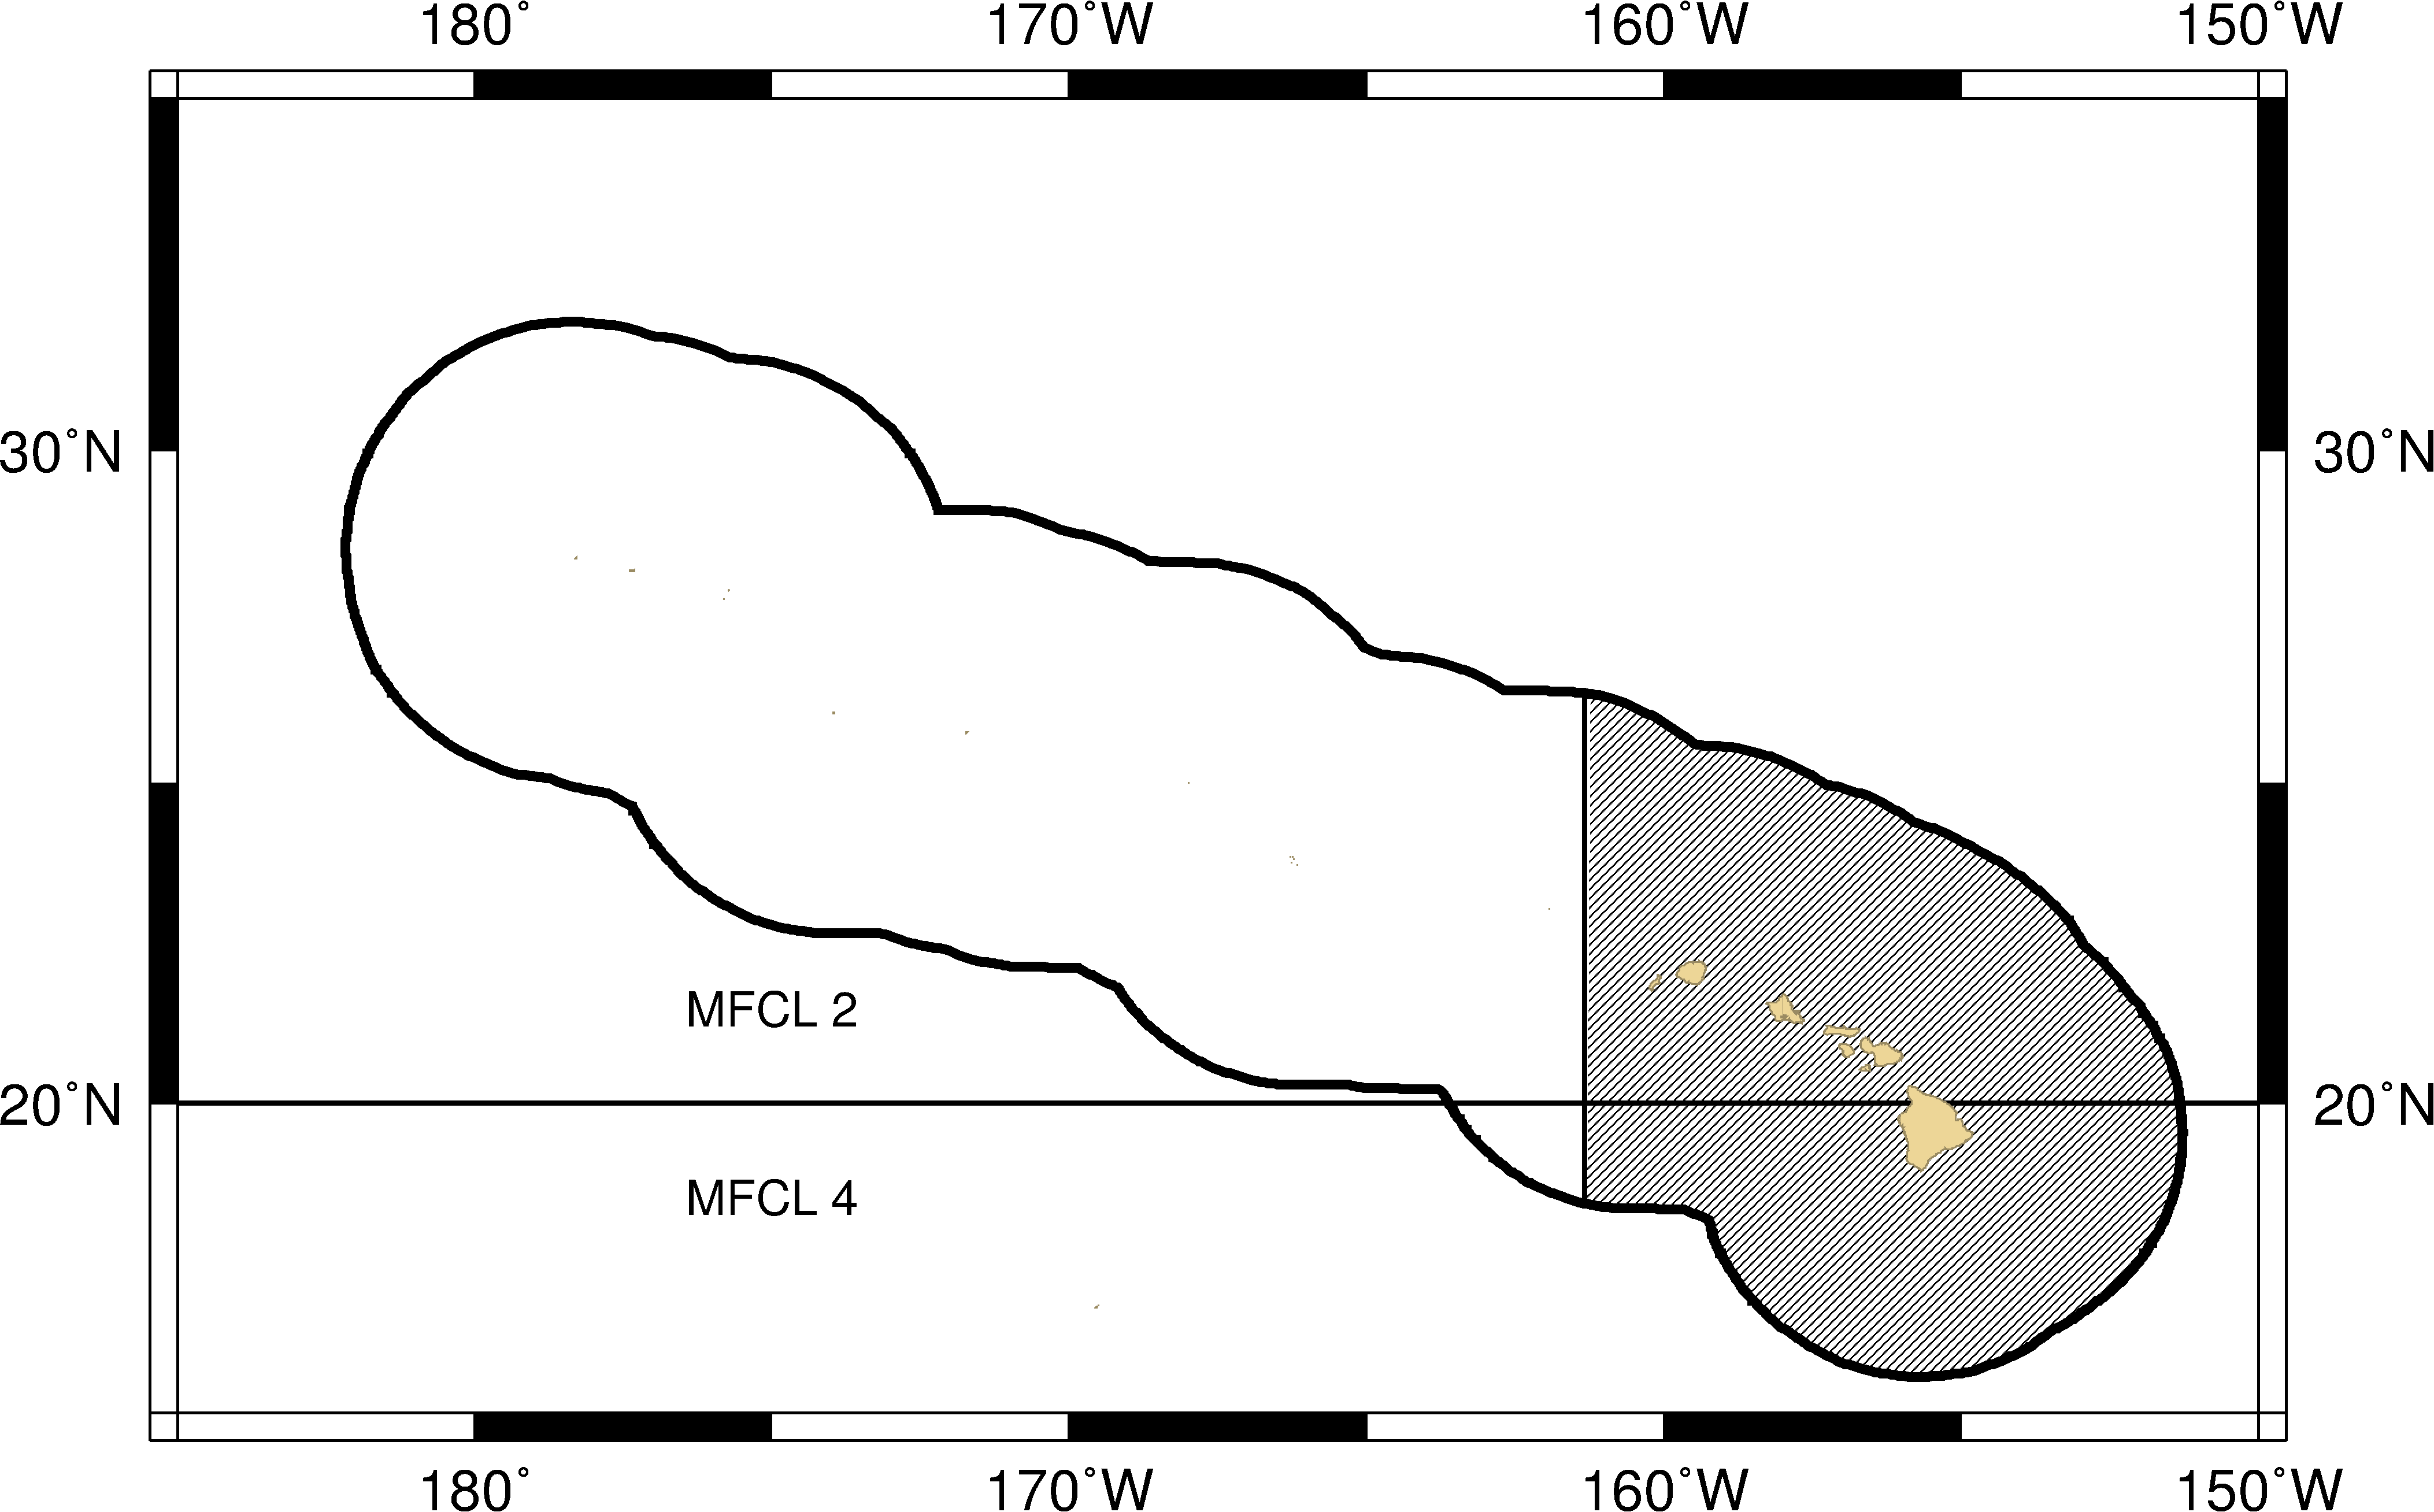
\includegraphics[width=\textwidth]{./graphics/HI_regions.png}
\caption{\label{fig:mhimap}
The United States Exclusive Economic Zone around the Hawaiian
Archipelago. The Main Hawaiian Islands lie in the shaded area at the
extreme east of the EEZ. The line at 20\deg{N} latitude is the
boundary between WCPFC stock assessment regions 2 and 4. See text for
full explanation.
}
\end{center}
\end{figure}

This paper presents an assessment of the stock of yellowfin tuna
residing in the MHI that may be of use to fishery managers in Hawaii
in addressing questions about the effects of the fishery on the
stock. The general approach is to adopt a state-space variant of
the surplus production model  (Schaefer, 1954). 
The model has several novel features.
Fishing mortality, the proportion of the population harvested each
year, is represented as a random walk (Nielsen and Berg, 2014).
Biomass estimates from the 2014 WCPFC yellowfin stock assessment
(Davies, et al. 2014) can be used as indices of abundance.
The logistic parameters of the surplus production model are
reparameterized to estimate parameters of direct relevance to fishery
management. State transitions are represented as random effects.


\section*{Model development}
\label{sec:models}
State-space models separate variability in the biological
processes in the system (transition model)
from errors in observing features of interest
in the system (observation model).

The general form of the transition model is
\begin{equation}
\alpha_t=T(\alpha_{t-1}) + \eta_t
\end{equation}
where $\alpha_t$ is the state at time $t$ and 
the function $T$ embodies the dynamics mediating the
development of the state at time $t$ from the state at the previous
time with random process error, $\eta_t$.

Stock dynamics follow the classic Schaefer differential equation:
\begin{equation}
\label{eqn:ischaefer}
\frac{dN}{dt} = rN(1-\frac{N}{K}) - FN
\end{equation}
where $N$ is the biomass of YFT in the MHI (mt), 
$r$ is the logistic growth rate (\peryr),
$K$ is the asymptotic biomass (mt), and
$F$ is the total fishing mortality (\peryr) in the MHI.

The state space transition equation is developed by solving
(\ref{eqn:ischaefer}) analytically from one time to the next and
applying a random error.
\begin{equation}
\label{eqn:intschaeferA}
N_t = \frac{K(r-\bar{F}_t)}{\frac{K(r-\bar{F}_t)}{N_{t-\Delta t}}e^{-\Delta
t(r-\bar{F}_t)}-re^{-\Delta t(r-\bar{F}_t)} -r} \cdot e^{\eta_t};
\quad \eta_t\sim N(0,\sigma^2_N)
\end{equation}
where 
and $\eta_t \sim N(0,\sigma_N)$ is a process error expressing
variability in population dynamics
and $\bar{F}_t$ is the total fishing mortality exerted by all gears, i. e.,
$$
\bar{F}_t =\sum_{g=1}^n F_{g,t}.
$$

The logarithm of fishing mortality for each gear is assumed to
follow a random walk with normal increments, as suggested by Berg and
Nielsen (2014).
\begin{equation}
\label{eqn:Fwalk}
\log F_{g,t} = \log F_{g,t-1} + \xi_t;\quad \xi_t\sim
N(0,\sigma^2_F)
\end{equation}
where  $\sigma^2_F$ is a process error expressing the year to year
variability in fishing mortality.

The index abundance assumes that the biomass of YFT in the MHI
is approximately proportional to some index which is independent of
the data analyzed in the model,
\begin{equation}
\log N_t - \log (Q\cdot I_t) = \omega_t;\quad \omega_t\sim N(0,\sigma^2_I)
\label{eqn:index}
\end{equation}
where
$I_t$ is the index at time $t$,
$Q$ is the estimated ratio of the MHI population size to the index,
and $\sigma^2_I$ is a process error representing the difference
between the MHI biomass and the abundance index. 
Conventional fishery independent methods such as acoustic or trawl
surveys are not applicable to tunas. 
Biomass estimates from the most recent WCPFC stock
assessment (Davies, et al. 2014) are convenient potential abundance
indices. The assessment method used by the
WCPFC is spatially structured and estimates biomass in several regions
in the pacific. The boundary between two of these
regions passes directly through the MHI (Figure~\ref{fig:mhimap}).
Both regions were evaluated as abundance indices.

The logistic parameters $r$ and $K$ are notoriously difficult to estimate
accurately in a surplus production model, 
so a parameter substitutions were used. 
Maximum sustainable yeld
(MSY, $\MSY$) and fishing mortality at MSY ($\Fmsy$) are commonly used
fishery reference points and are simple functions of $r$ and $K$.
Therefore $\MSY$ and $\Fmsy$ were
estimated directly and substituted in (\ref{eqn:intschaeferA}) as
$r=2\Fmsy$ and $K=\frac{4\MSY}{r}$.

Carruthers and McAllister (2011) recommend use of Bayesian priors for the
logistic growth parameter $r$ in equation~(\ref{eqn:ischaefer}). They
suggest $\tilde{r} = 0.486$ with a standard deviation of $\sigma_r = 0.046$
and coefficient of variation of ${\rm cv}=0.094$ for Atlantic YFT.
A lognormal prior on $r$ was implemented with 
$\tilde{r} = 0.486$ and $\sigma_r = 0.8$.
\begin{equation}
\log r - \log \tilde{r} = \rho ;\quad \rho\sim N(0,\sigma^2_r)
\end{equation}
which is a somewhat ``looser'' constraint on the estimate of $r$.
$\rho$ becomes a component of the likelihood
(equation~\ref{eqn:likelihood}).

All process errors are assumed to have the same distribution
$N(0,\sigma^2_P)$; $\sigma_N$,$\sigma_F$, and $\sigma_I$ are assumed
to be equal and estimated as a global process error with variance
$\sigma^2_P$.

The general form of the observation model is
\begin{equation}
x_t = O(\alpha_t) + \varepsilon_t
\end{equation}
where the function $O$ describes the measurement process with
error $\varepsilon$ in observing the population.

Predicted catch, $\widehat{C}_{g,t}$, for each gear is the product of
estimated fishing mortality and the biomass.
\begin{equation}
\widehat{C}_{g,t} = F_{g,t}\cdot\Bigl(\frac{N_{t-\Delta
t}+N_t}{2}\Bigr) \cdot e^{\varepsilon_t}
\label{eqn:obs1}
\end{equation}
where the biomass is  the average
biomass over the time step (Quinn and Deriso, 1999), and
$\varepsilon_t$ is a ``zero-inflated'' log normal likelihood given by
\begin{equation}
  \log \varepsilon_t = \left\{
    \begin{array}{r@{\;:\quad}l}
       C_{g,t} > 0 &
(1-p_0)\cdot\bigg(\log\frac{1}{\sqrt{2\pi\sigma^2_Y}}
          -\Bigl(\frac{\log
C_{g,t}-\log\widehat{C}_{g,t}}{\sigma_Y}\Bigr)^2\bigg)\\
       C_{g,t} = 0 & p_0 \cdot\log \frac{1}{\sqrt{2\pi\sigma^2_Y}}\\
    \end{array}
  \right.
\end{equation}
where $C_{g,t}$ is the observed catch for gear $g$ at time $t$,
$\sigma_Y$ is the observation error and
$p_0$ is the proportion of observed catch observations equal to zero.
This proportion may be estimated or fixed at a constant value. 
%For current analysis, it is fixed at $p_0 = 0.15738$ as computed from the data.
% line 186, file issams.cpp, prop_zero =  0.4918 0 0 0.098361 0.19672, tprop_zero = 0.15738


\begin{table}
\caption{Complete list of estimated and computed parameters and model
constraints for 
the state-space surplus production model. There are 5 estimated parameters. 
For a model with 61 time steps and 4 gear types there are 305 random effects.
Values of non-estimated model variables, e.g.,  $r$ and $K$, are computed by
parameter substitution formulas.
There are three constraints.
}
\label{tab:allvars1}
\begin{center}
\begin{tabular}{ll}
\hline
Parameter & Definition\\
\hline
\hline
$\MSY$ & Maximum sustainable yield\\
$\Fmsy$& Fishing mortality at maximum sustainable yield\\
$Q$    & Abundance index proportionality constant\\
$\sigma_P$ & Global process error SD; $\sigma_P=\sigma_N=\sigma_F=\sigma_I$\\
$\sigma_Y$ & Observation error SD \\
\hline
$r$    & Instantaneous growth rate; $r=2F_{\MSY}$\\
$K$    & Asymptotic population size; $K=\frac{4\MSY}{r}$\\
\hline
$p_0$  & Proportion of zero catch observations;\\
       & fixed at 0.04918\\
$\tilde{r}$ & An {\it a priori} assumed value for $r$\\
            & fixed at $\tilde{r}=0.486$ (Carruthers and McAllister, 2011)\\
$\sigma_r$  & Assumed standard deviation of $r$ around its prior;\\
            & fixed at $\sigma_r=0.8$.\\
\hline
\end{tabular}
\end{center}
\end{table}



%{\bf Estimation.} 
The model states, $N_t$ and $F_{gt}$ are assumed to be random
effects (Skaug and Fournier, 2006). Model parameters are estimated by
maximizing the joint likelihood of the random
effects, observations, and prior likelihood.
\begin{equation}
\label{eqn:likelihood}
L(\theta,\alpha,x)=
\prod^m_{t=2}\big[\phi\big(\alpha_t-T(\alpha_{t-1}), \Sigma_\eta\big)\big]\cdot
\prod^m_{t=1}\big[\phi\big(x_t-O(\alpha_t),
\Sigma_\varepsilon\big)\big]\cdot\rho
\end{equation}
Here, $m=61$, the number of time steps in the catch time series and
$\theta$ is a vector of model parameters (Table~\ref{tab:allvars1}).
The model is implemented in ADMB-RE (Fournier et al, 2012).
The actual number of
parameters to be estimated depends on the model configuration,
specified by phase flags in the input file. 
All computer code, data files, and draft reports in support of this
analysis can be found at Github:
\url{https://github.com/johnrsibert/XSSA.git}.

\section*{Results}


\begin{table}
\caption{Yada yada
}
\label{tab:ests1}
\begin{center}
\begin{tabular}{lrrrr}
\hline
 &\multicolumn{4}{c}{Index Region}\\
\cline{2-5}
Estimate &               2&              4&            None& None\\
\hline
\hline
$\MSY$       & 1384.7700000000& 979.9600000000& 5533.8000000&1011.840000000\\
$\Fmsy$      &    0.1159930000&   0.9199500000&    0.4359210& 0.248501000\\
$Q$            &    0.0720595000&   0.0007741100&    0.0500016& 0.050001600\\
$\sigma_P$    &    0.2330650000&   0.2337410000&    0.3208980& 0.318883000\\
$\sigma_Y$    &    0.3974540000&   0.3946970000&    0.3495700& 0.351795000\\
\hline
$-\log L$ &  199.0340000000& 192.6540000000&  270.8720000& 195.105000000\\
$n$       &    5.0000000000&   5.0000000000&    4.0000000& 4.000000000\\
$|G|_{max}$ &    0.0000919767&   0.0000478966&    0.1377480& 0.000013202\\
\hline
$r$          &    0.2319860000&   1.8399000000&    0.8718420& 0.497003000\\
$K$          &23876.7000000000&2130.4600000000&25389.0000000&8143.520000000\\
\hline
$p_0$         &    0.0491800000&   0.0491800000&    0.0491800& 0.049180000\\
$\tilde{r}$  &    0.4860000000&   0.4860000000&    0.4860000& 0.486000000\\
$\sigma_r$   &    0.8000000000&   0.8000000000&    0.8000000& 0.200000000\\
\hline
$\log\sigma_P$ &   -1.4564400000&  -1.4535400000&   -1.1366300& -1.142930000\\
$\log\sigma_Y$&   -0.9226750000&  -0.9296360000&   -1.0510500& -1.044710000\\
$\log\MSY$  &    7.2332900000&   6.8875100000&    8.6186300& 6.919520000\\
$\log\Fmsy$  &   -2.1542200000&  -0.0834354000&   -0.8302940& -1.392310000\\
\hline
\end{tabular}
\end{center}
\end{table}


%%%%%%%%%%%%%%%%%%%%%%%%%%%%%%%%%%%

%\vspace{4ex}
\clearpage
\singlespacing
\noindent {\bf Acknowledgements.}
This work was initiated under a contract from the Western Pacific Regional Fisheries
Managment Council. I thank the Council for its generous support and
Council Staff Paul Dalzell and Eric Kingma for encouraging me to
actually take on this challenging project and for their on-going
collaboration. Special thanks
to David Itano for sharing insights into the small-boat fisheries in Hawaii,
to Reginald Kokubun State of Hawaii, Division of Aquatic Resources,
Departmemnt of Land and Natural Resources for supplying catch report
data from the Commercial Marine Landings data base,
to Keith Bigelow and Karen Sender of NOAA Pacific
Island Fisheries Science Center for supplying logbook reporting data and
from the PIFSC data base.
Thanks also to John Hampton of the Secretariat of the Pacific
Community, Oceanic Fisheries Programme, for making available \MFCL\
output files from the latest Western and Central Pacific
Fisheries Commission yellowfin tuna stock assessment, and to Nick
Davies for sharing R scripts and advice on interpreting those files.


\section*{References}
{\parindent=0cm \small
\everypar={\hangindent=2em \hangafter=1}\par
%\doublespacing
Carruthers, T. and M. McAllister. 2011.
Computing prior probability distributions for the
intrinsic rate of increase for Atlantic tuna and
billfish using demographic methods.
Collect. Vol. Sci. Pap. ICCAT, 66(5): 2202-2205.

Davies, N., S. Harley, J. Hampton, S. McKechnie. 2014. Stock
assessment of yellowfin tuna in the western and central pacific ocean.
WCPFC-SC10-2014/SA-WP-04.

Fournier, D. A., H.J. Skaug, J. Ancheta, J.Sibert, J. Ianelli, 
A. Magnusson, M. N. Maunder, A. Nielsen. 2012. AD Model Builder:
using automatic differentiation for for statistical inference of highly
parameterized complex nonlinear models. Optimization Methods and
Software 27, 233–249.

Nielsen, A., C. Berg. 2014. Estimation of time-varying selectivity
in stock assessments using state-space models. Fisheries Research
158:96-101.

%Murray, J. D. 1993. Mathematical biology. Second Edition.
%Springer-Verlag. 767pp.

Quinn, T, R. Deriso. 1999. Quantitative fish dynamics. Oxford
University Press, New York.

Rooker, J. 2016.

Schaefer, M. B. 1954. Some aspects of the dynamics of populations
important to the management of the commercial marine fisheries. IATTC
Bull. 1(2):27-56.

Senina, I., J. Sibert, P. Lehodey  2008. Parameter estimation for
basin-scale ecosystem linked population models of large pelagic
predators: Application to skipjack tuna.  Prog. Oceanogr. 78:319-335.

Senina, I.,  P. Lehodey, B. Calmettes, S. Nicol, S. Caillot,
J. Hampton and P. Williams. 2015.
SEAPODYM application for yellow tuna in the Pacific Ocean.
WCPFC-SC11-2015/EB-IP-01.


Skaug, H., Fournier, D., 2006. Automatic approximation of the marginal
likelihood in non-Gaussian hierarchical models. Computational
Statistics \& Data Analysis 51, 699–709.

Wells, D., J. Rooker, D. Itano. 2012.  Nursery origin of yellowfin
tuna in the Hawaiian Islands. Mar. Ecol. Prog. Ser. 461:187-196. 
\par}

\clearpage


%\numberwithin{figure}{section}
\appendix
\section*{Data preparation}
\label{sec:data}

\subsection*{Catch data}

\begin{figure}
\begin{center}
%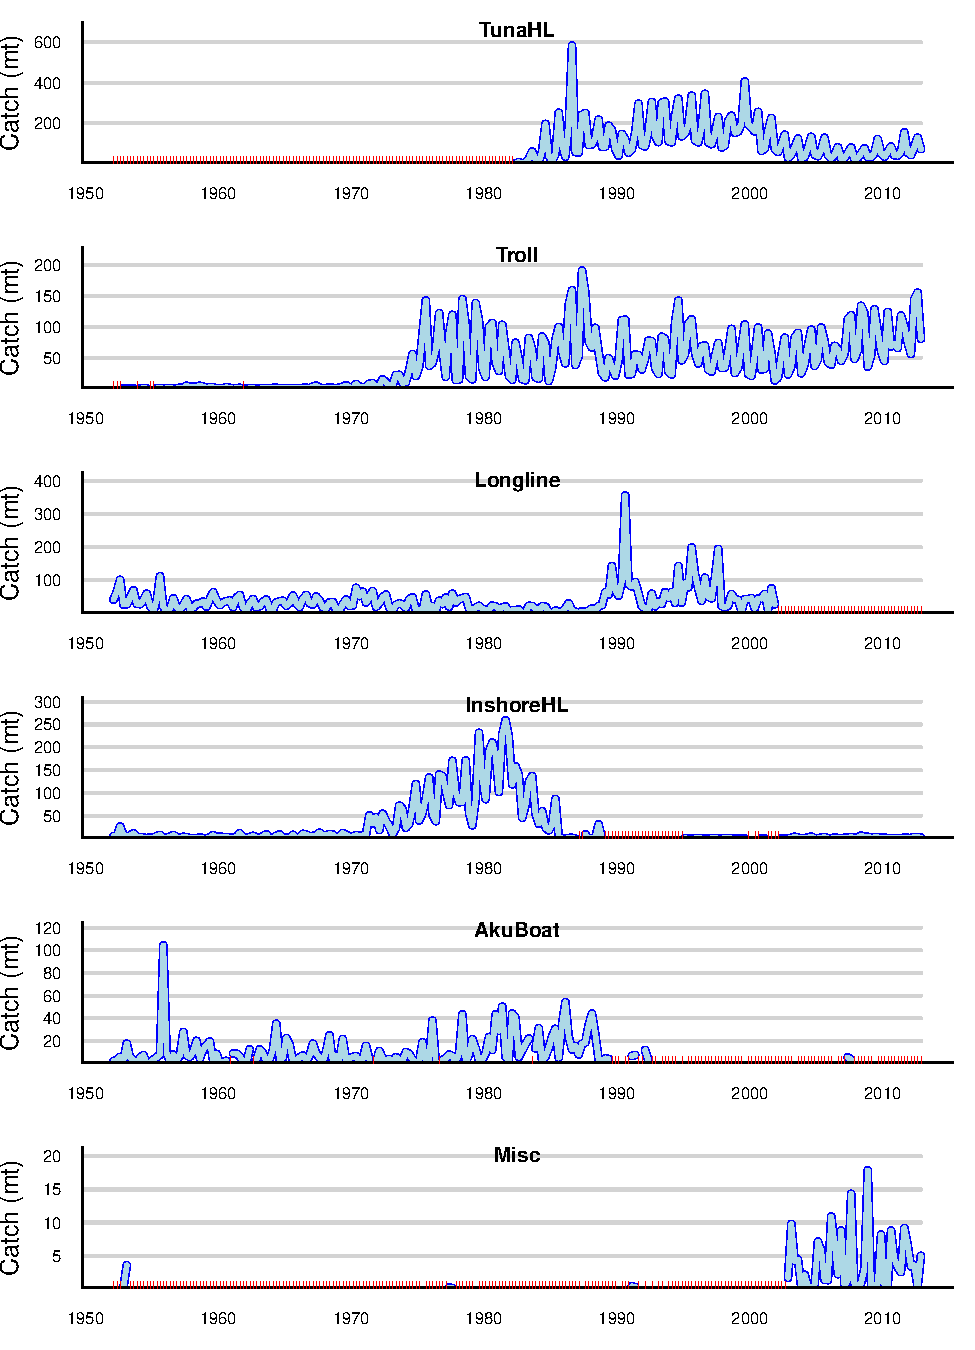
\includegraphics[width=\textwidth]{./graphics/CML.pdf}
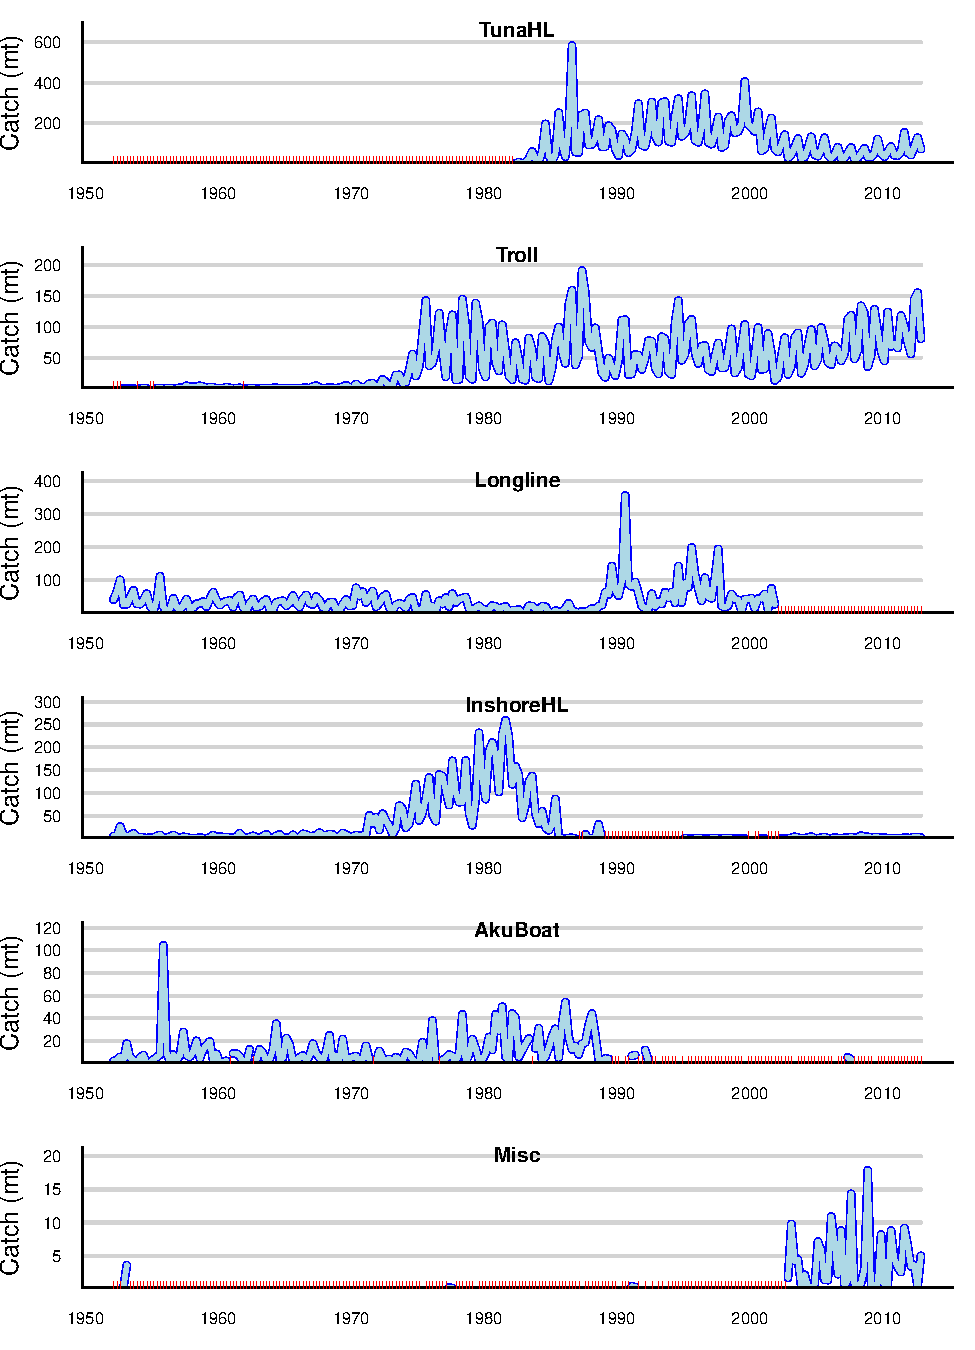
\includegraphics[height=0.8\textheight]{./graphics/CML.pdf}
\caption{\label{fig:CMLdata}
Yellowfin catch in metric tonnes by principle fisheries operating in
the Main Hawaiian Islands from the State of Hawaii Commercial Marine
Landings Data.
The red tick marks on the abscissa indicate quarters where reported
catches were zero.
}
\end{center}
\end{figure}


%Commercial Marine Landings, Division of Aquatic Resources, Dept. of Land and Natural Resources, State of Hawaii
The State of Hawaii Department of Land and Natural Resources
Commercial Marine Landings data base (CML) from 1949 through 2014 is
the primary source of data used in this analysis. These document the
continuous 65 year history of commercial fishing in Hawaii.


The CML catch reports were aggregated into the following gear categories:
``Aku boat'', ``Bottom/inshore HL'', ``Longline'',  ``Troll'', ``Tuna
HL'', ``Casting'', ``Hybrid'',  ``Shortline'', ``Other'', and
``Vertical line''.
For this analysis catches by ``Casting'', ``Hybrid'',
``Shortline'', ``Other'', and ``Vertical line'' are combined into a new
category, ``Misc''. Landing in the ``Misc'' category are highest after
year 2000 and less than 20 mt, i.e. 2\% of the total landings.
The catch time series for the CML data are shown in
Figure~\ref{fig:CMLdata}.
The ``Bottom/inshore HL'' and ``Tuna HL'' are both handline gears and
the data for these two gear types were combined at the suggestion of
the CML database administrator.
The ``Aku Boat'' gear type refers to storied Japanese-style pole and
line fishery that operated in Hawaii through th 1980s. This fishery
collapsed because of lack of access to bait and the closure of the only
cannery in Honolulu. The Aku Boats target skipjack tuna 
({\it Katsuwonus pelamis}), but yellowfin were occasionally landed as
incidental catch.
Some time series contain sustained periods of zero catch which
reflect the development and subsequent shift away from a specific
gear type. It is assumed that these declines in catches represent
``collapse'' of a fishery due to social and economic factors rather than
to a decline of YFT stocks.
Similarly, some time series are punctuated by brief episodes (one or two quarters in
length) of zero catches. Again, it is assumed that these zero catches
are not caused by low stock size.


The Hawaii-based longline fishery began a rapid expansion in the late
1980s, and the United States National Oceanic and Atmospheric Administration (NOAA)
began to collect data from the longline fleet under a
federally mandated logbook program in 1990. The CML longline data were
augmented by NOAA longline log sheet data from 1995 through 2013.
NOAA distinguishes deep sets, targeting bigeye tuna ({\it Thunnus
obesus}), and shallow sets,
targeting swordfish ({\it Xiphias gladius}) in the data. 
The CML data do not distinguish between deep and shallow sets.
Since the longline fleet ranges widely in the North Pacific Ocean,
only catches reported in the United States EEZ around Hawaii east of
162\deg{W} longitude were included in the data.
Figure~\ref{fig:hdarnoaaLLTS} shows the correspondence between the
CML and NOAA time series. The combined deep plus shallow catches from
NOAA align fairly well with the overlapping CML data. The simple
average of the CML data with the combined NOAA deep plus shallow data
appears to be roughly the same trajectory as the
constituent time series. Yellowfin is currently considered an incidental catch
in the longline fishery.

\begin{figure}
\begin{center}
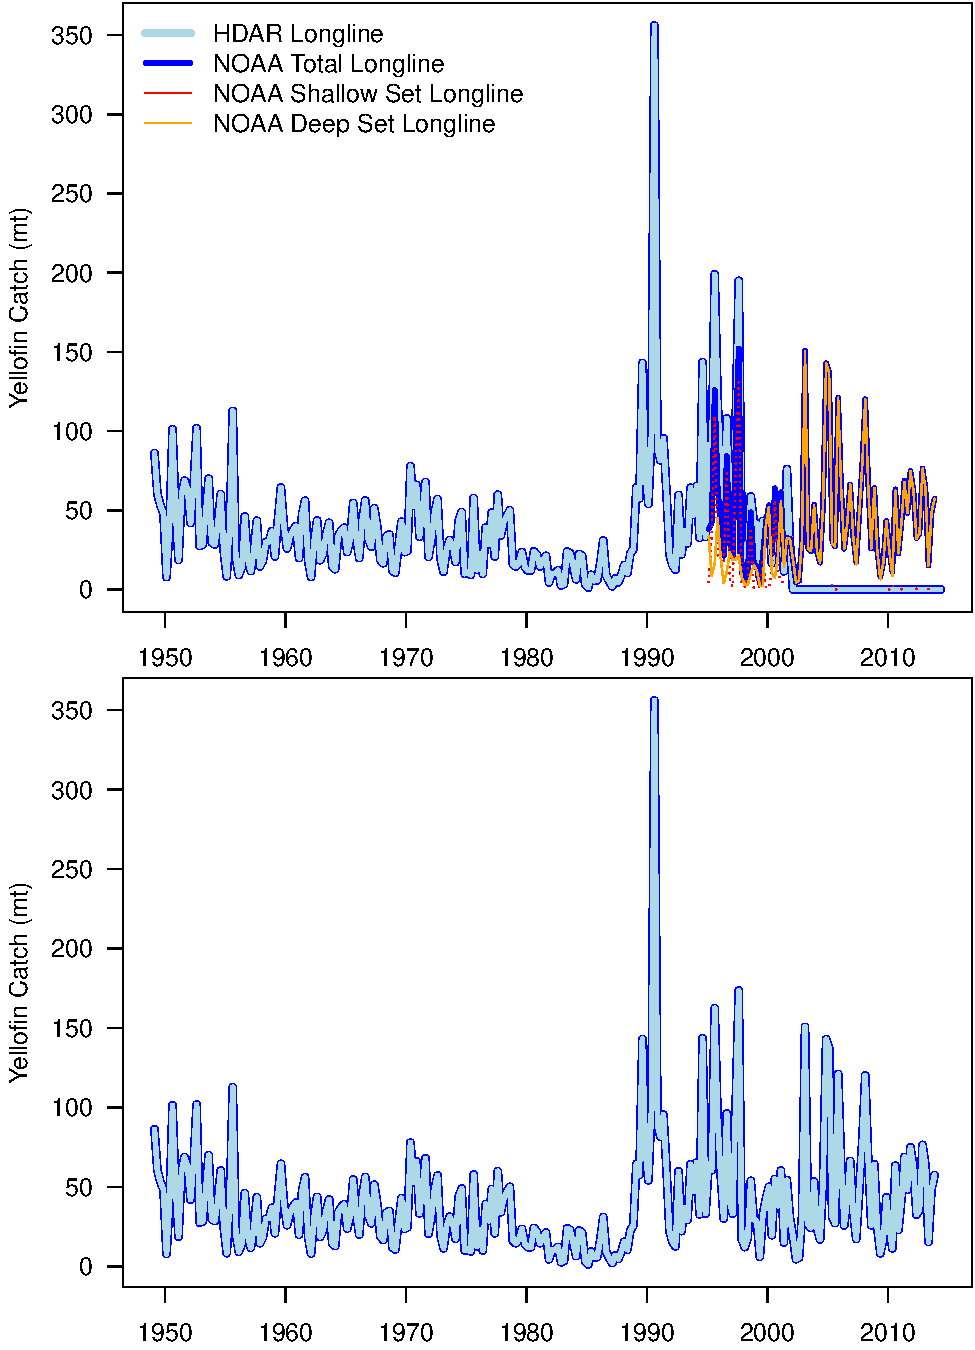
\includegraphics[height=0.8\textheight]{./graphics/hdar_noaa_LL_ts.pdf}
%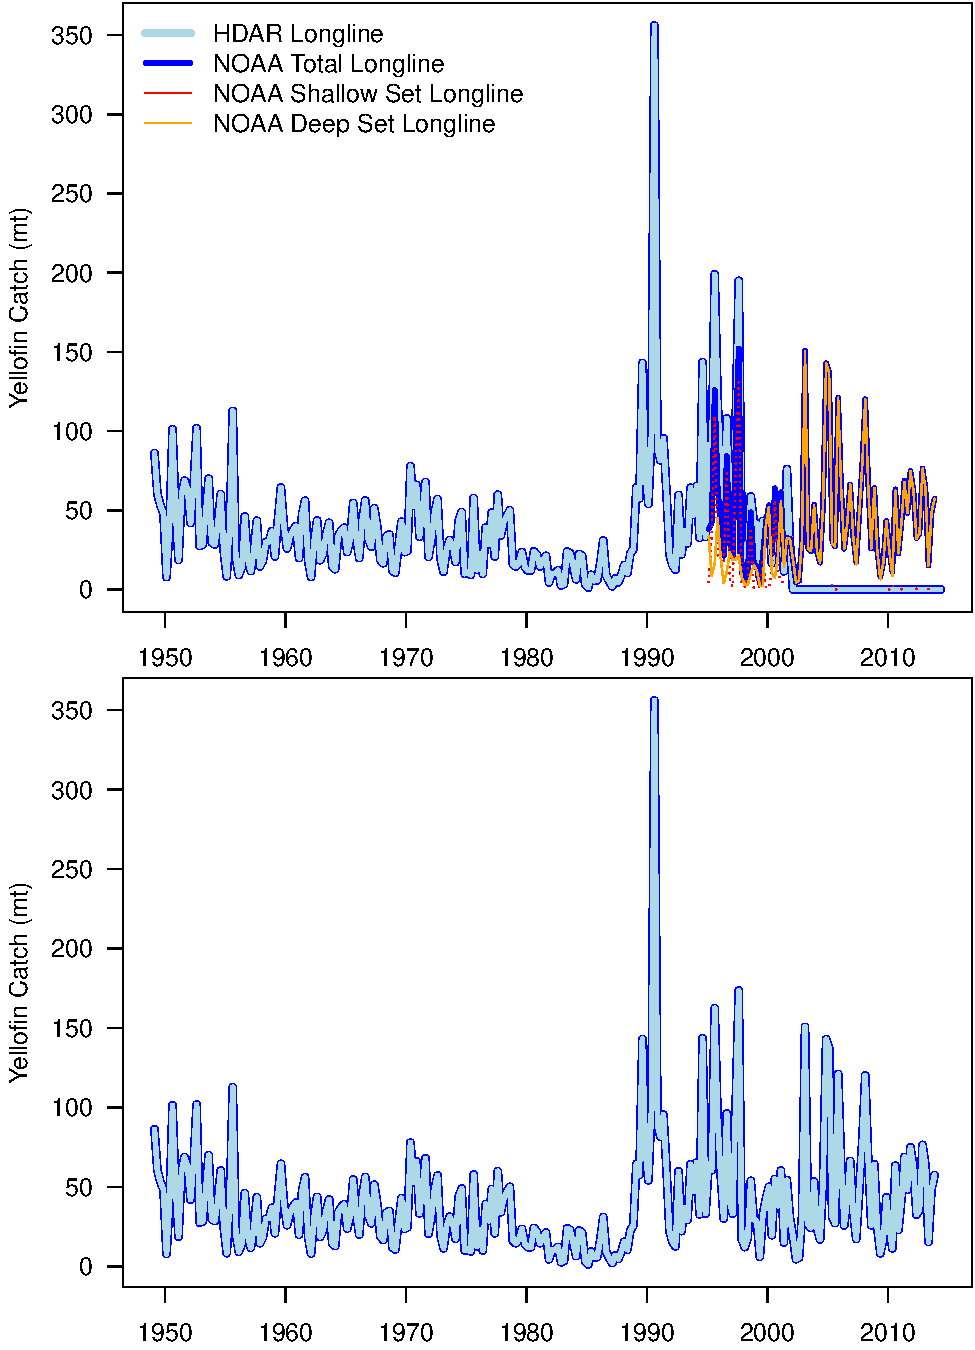
\includegraphics[width=\textwidth]{./graphics/hdar_noaa_LL_ts.pdf}
\caption{\label{fig:hdarnoaaLLTS}
Comparison between CML and NOAA longline time series. The upper panel
shows the NOAA deep and shallow set data superimposed on the HDAR
data. The lower panel shows the time series produced by a simple
average of the CML data and the sum of the NOAA deep and shallow
catches.}
\end{center}
\end{figure}

are the sources of catch data used in this assessment. Catch data from
both sources were initially aggregated by quarter of the calendar year for the
relevant time periods 
All catch time series exhibit annual cycles suggesting seasonal
signals in the catches by all gears. To avoid the need to estimate
autocorrelation matrices for each time series and to minimize the
number of zero catch observations, the quarterly time series were
aggregated into the annual time series shown in Figure~\ref{fit:data}
and used in this analysis.

\begin{figure}
\begin{center}
%                                         graphics/4_gear_catch_history_a.pdf
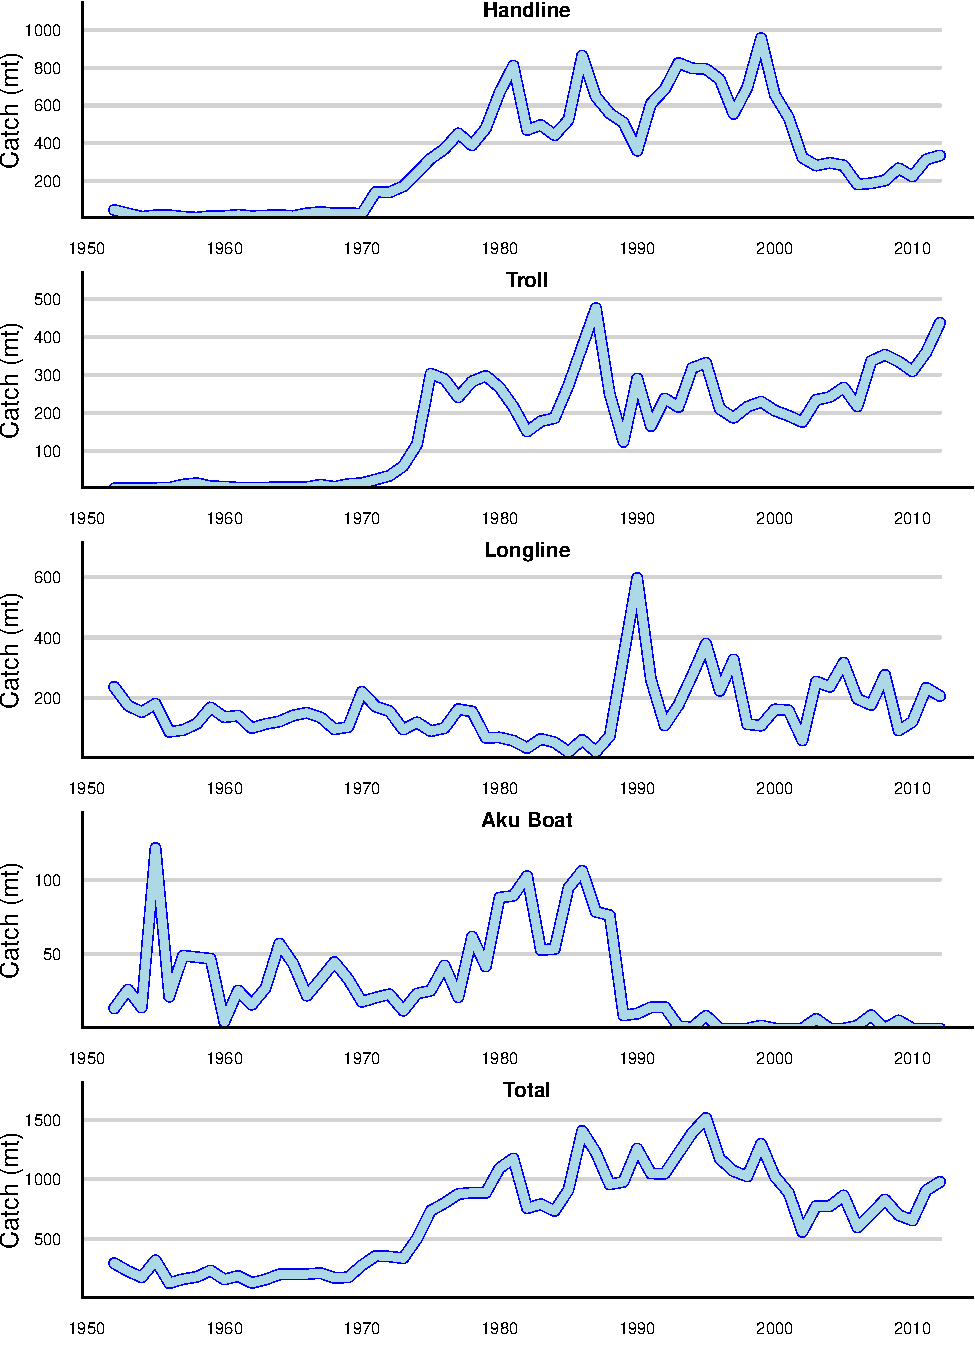
\includegraphics[height=0.8\textheight]{./graphics/4_gear_catch_history_a.pdf}
\caption{\label{fig:data}
Four gear type catch time series used in the assessment model.
}
\end{center}
\end{figure}

\clearpage
\subsection*{Off line coupling}
The MHI assessment model could be 1coupled to two different models of
the WCPO yellowfin stocks, \MFCL\ and \SD. Both models are age
structure and spatially resolved and have been applied to YFT.
The spatial resolution of the \SD\ YFT model is 1\deg{} whereas the
\MFCL\ yellowfin assessment divides the WCPO into 9 regions to facilitate
incorporation of tagging data and to improve mortality estimates
Figure~\ref{fig:mfclregions}.
The spatial resolution of the \SD\ model would make it an ideal
candiate for computing an index of abundance, but the model is still
under active development. In contrast the 2014 \MFCL\ assessment has
been officially adopted as the best available assessment.

\begin{figure}
\begin{center}
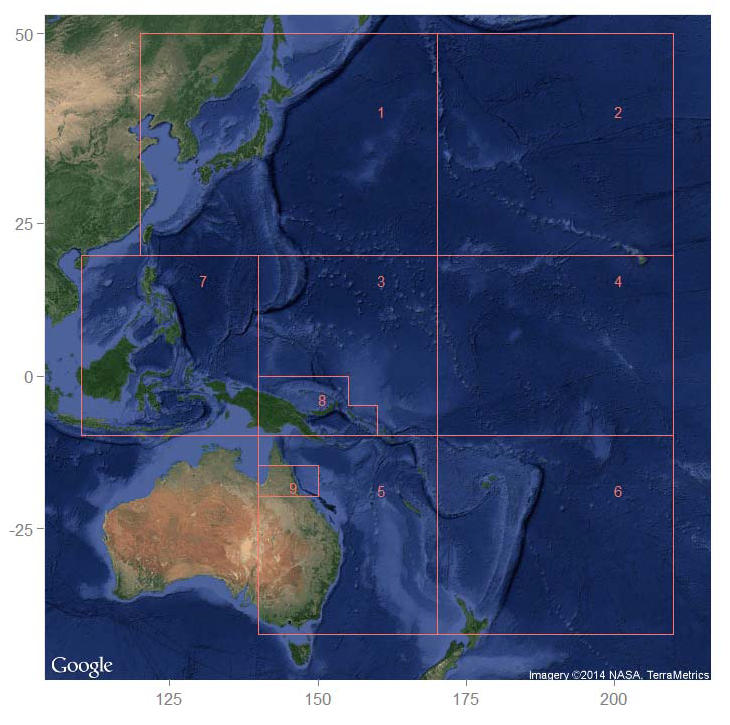
\includegraphics[width=0.8\textwidth]{./graphics/MFCLregions.png}
\caption{\label{fig:mfclregions}
Regional structure used in the 2014 WCPFC YFT stocks assessment.
}
\end{center}
\end{figure}

Unfortunately the \MFCL\ regions split the MHI between regions 2 and 4. 
Both regions were evaluated as abundance indices.

\begin{figure}
\begin{center}
\begin{tabular}{lr}
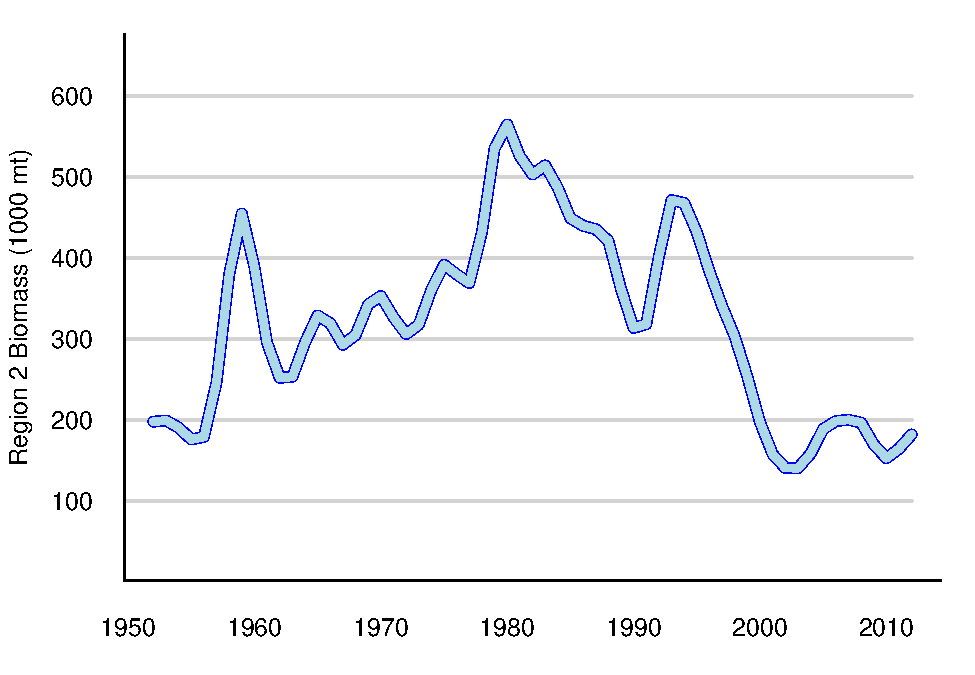
\includegraphics[width=0.50\textwidth]{./graphics/annual_region_2_biomass.pdf} &
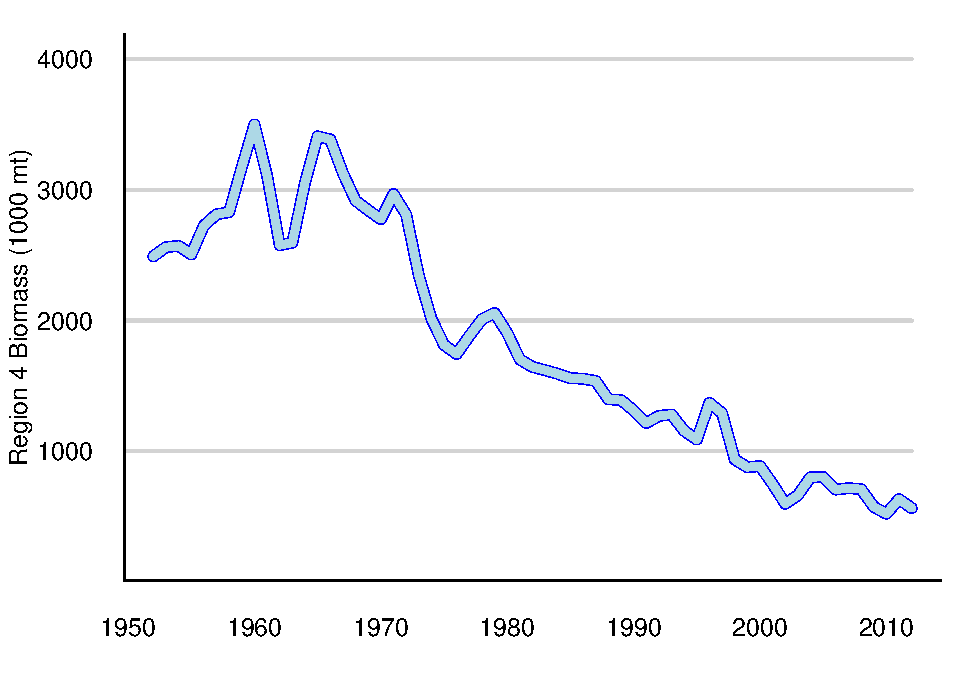
\includegraphics[width=0.50\textwidth]{./graphics/annual_region_4_biomass.pdf} \\
\end{tabular}
\end{center}
\caption{Estimated biomass trends in \MFCL\ regions 1 and 2 (Davies, et al. 2014).
\label{fig:mfclbiomass}
}
\end{figure}


 
\end{document}

